\documentclass[twocolumn]{article}

\usepackage[utf8]{inputenc}
\usepackage{graphicx}
\usepackage{amssymb}
\usepackage{amsmath}
\providecommand{\pr}[1]{\ensuremath{\Pr\left(#1\right)}}
\providecommand{\cbrak}[1]{\ensuremath{\left\{#1\right\}}}

\title{Assignment 4}
\author{Gollapudi Sasank CS21BTECH11019}

\begin{document}
\maketitle
\section*{Question : }
A die is thrown 1000 times with frequencies for outcomes 1,2,3,4,5 and 6 as given in the following table:
\begin{table}[ht]
\begin{tabular}{|c|c|c|c|c|c|c|}

\hline
\textbf{Outcome} & $1$ & $2$ & $3$ & $4$ & $5$ & $6$ \\

\hline
\textbf{Frequency}&  $179$ & $150$ & $157$ & $149$ & $175$ & $190$ \\

\hline

\end{tabular}
\centering
\caption{}
\label{table:table 1}
\end{table}\\
Find the probability of getting each outcome.
\section*{Solution : }
Let Rolling of a dice be the experiment and the random variable $X \in \cbrak{1,2,3,4,5,6}$  denote the outcome of the experiment.\\
Where $X = i $ denote the occurence of outcome $i$ in the experiment for $ i = 1,2,3,4,5,6 $
\begin{align}
\pr{X = 1} = \frac{179}{1000} = 0.179 \\
\pr{X = 2} = \frac{150}{1000} = 0.150 \\
\pr{X = 3} = \frac{157}{1000} = 0.157 \\
\pr{X = 4} = \frac{149}{1000} = 0.149 \\
\pr{X = 5} = \frac{175}{1000} = 0.175 \\
\pr{X = 6} = \frac{190}{1000} = 0.190 
\end{align}

If we plot PMF(Probability Mass Function) of theoretical and experimental data we get the following bar graph 

\begin{figure}[h]
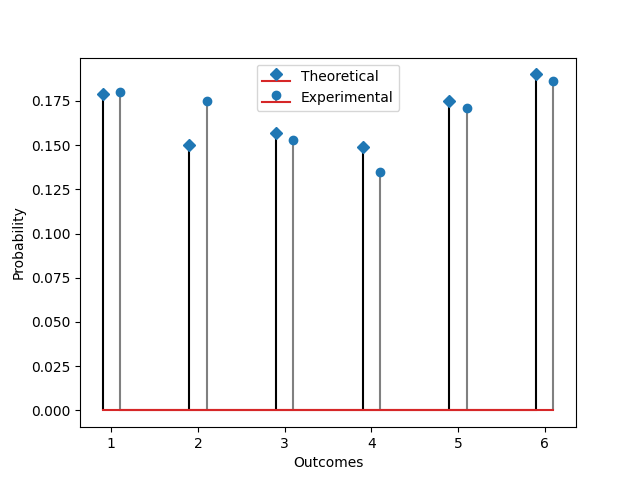
\includegraphics[width=\columnwidth]{fig1.png}
\caption{PMF of theoretical and experimental data}
\label{Fig 1}

\end{figure}
For a fair die probability of each number $ = \frac{1}{6} $ \\
\begin{align}
\Rightarrow
\pr{X = i}  = \frac{1}{6} 
\end{align}
 for i = 1,2,3,4,5,6
\end{document}